\documentclass{beamer}

\usepackage[utf8]{inputenc}
\usepackage[spanish]{babel}
\usepackage{multicol}
\usepackage{graphicx}
\usepackage{hyperref}
\usepackage{svg}
\usepackage{amsmath}

\setbeamertemplate{navigation symbols}{}
\usetheme{Montpellier}
\usecolortheme{crane}
\setbeamertemplate{itemize subitem}[circle]
%\beamersetuncovermixins{\opaqueness<1>{25}}{\opaqueness<2->{15}}

\graphicspath{ {figures/} }

%Información para la portada
\title{Sensibilización SwL}
\author{Manuel Vidal García\\ Pablo \\ Miguel Rodríguez-Segade}
\date{\today}

\begin{document}

\begin{frame}
    \titlepage
\end{frame}

\begin{frame} \frametitle{Table of contents}
    \tableofcontents
\end{frame}

\section{Distribuciones}

\begin{frame}\frametitle{¿Qué es una distribución GNU/Linux?}

    \begin{center}
        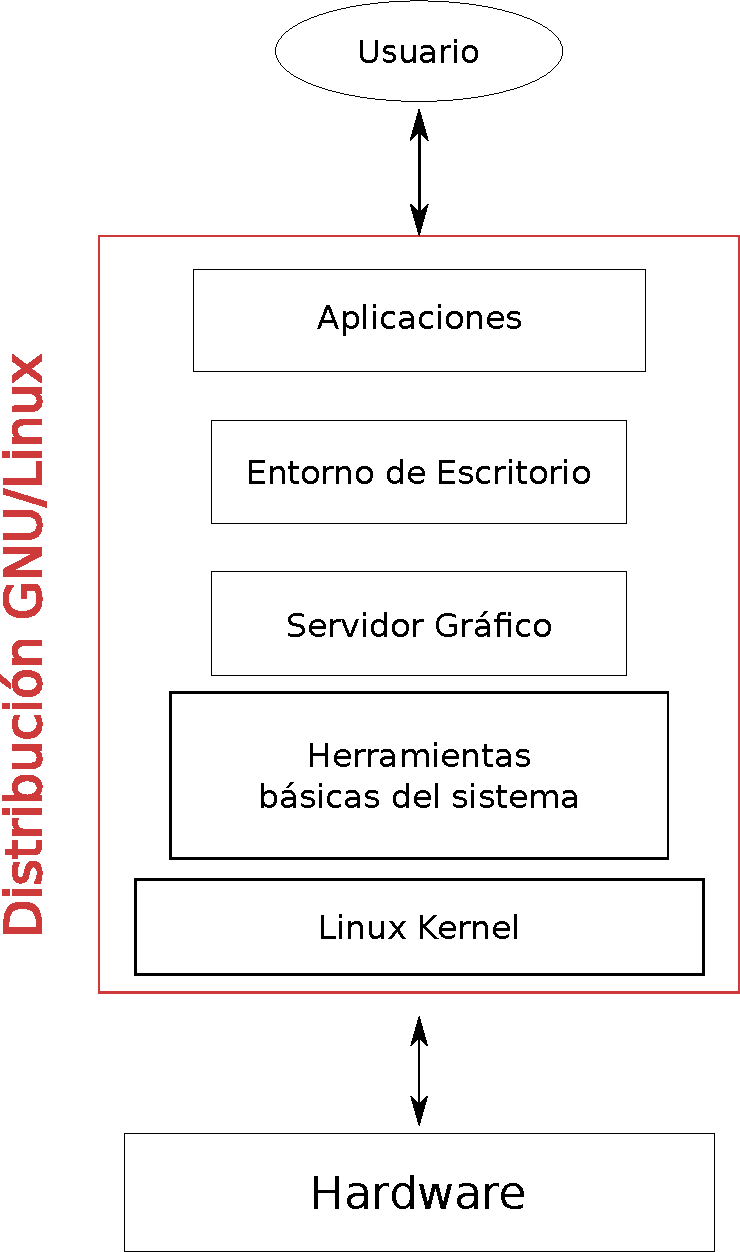
\includegraphics[ height=5.8cm, keepaspectratio]{esquemadistro.pdf}
    \end{center}

\end{frame}

\section{Arrancar desde el CD/USB}

\section{Probar la distribución}

\section{Instalador}

\section{Configuración básica}

\section{Primeros pasos}

\end{document}
